\documentclass{ximera}
\graphicspath{
{./}
{volumes/}
{arclengths/}
{centroids/}
{techniques/}
{applications/}
{series/}
{powerseries/}
{odes/}
{lessons/}
}
\usepackage{booktabs}

\newcommand{\bigmath}[1]{$\displaystyle #1$}
\newcommand{\choicebreak}{}
\newenvironment{type}{}{}
\newenvironment{notes}{}{}
\newenvironment{keywords}{}{}
\newcommand{\offline}{}
\newenvironment{comments}{\begin{feedback}}{\end{feedback}}
\newenvironment{multiplechoice}{\begin{multipleChoice}}{\end{multipleChoice}}
\title{Trigonometric Substitions}
%%%%%\author{Philip T. Gressman}

\begin{document}
\begin{abstract}
  We practice executing trigonometric substitutions.
\end{abstract}
\maketitle

\section*{(Video) Calculus: Single Variable}
\youtube{D_2N1OLQjyk}

\section*{Online Texts}
\begin{itemize}
\item \link[OpenStax II 3.3: Trigonometric Substitution]{https://openstax.org/books/calculus-volume-2/pages/3-3-trigonometric-substitution}
\item \link[Ximera OSU: Trigonometric Substitution]{https://ximera.osu.edu/mooculus/calculus2/trigonometricSubstitution/titlePage}
\item \link[Community Calculus 8.3: Trigonometric Substitution]{https://www.whitman.edu/mathematics/calculus_online/section08.03.html}
\end{itemize}


\section*{Examples}

\begin{example}
(c.f.~APEX Calculus Example 6.4.2) Compute the indefinite integral
\[ \int \frac{dx}{\sqrt{5 + x^2}}. \]
\begin{itemize}
\item The structure of this integrand is adapted to a trigonometric substitution of \wordChoice{\choice{secant}\choice{sine}\choice[correct]{tangent}} type, so we let $x = \sqrt{5} \answer{\tan \theta}$ (type out the word theta). This gives $dx = \sqrt{5} \answer{\sec^2 \theta}~d \theta$.
\item We use the identity $\sec^2 \theta = \tan^2 \theta + 1$, the quantity $5 + x^2$ can be rewritten using our substitution to equal $\answer{5 \sec^2 \theta}$. Therefore
\[ \int \frac{dx}{\sqrt{5+x^2}} dx = \int \answer{\sec \theta} \, d \theta = \answer{\ln | \sec \theta + \tan \theta|} + C. \]
(When writing out the indefinite integral, don't forget absolute values.)
\item We construct a reference triangle compatible with our substitution. In this case, that means we need a right triangle with an angle $\theta$ which satisfies $x/\sqrt{5} = \tan \theta$:
\begin{center}
\begin{image}
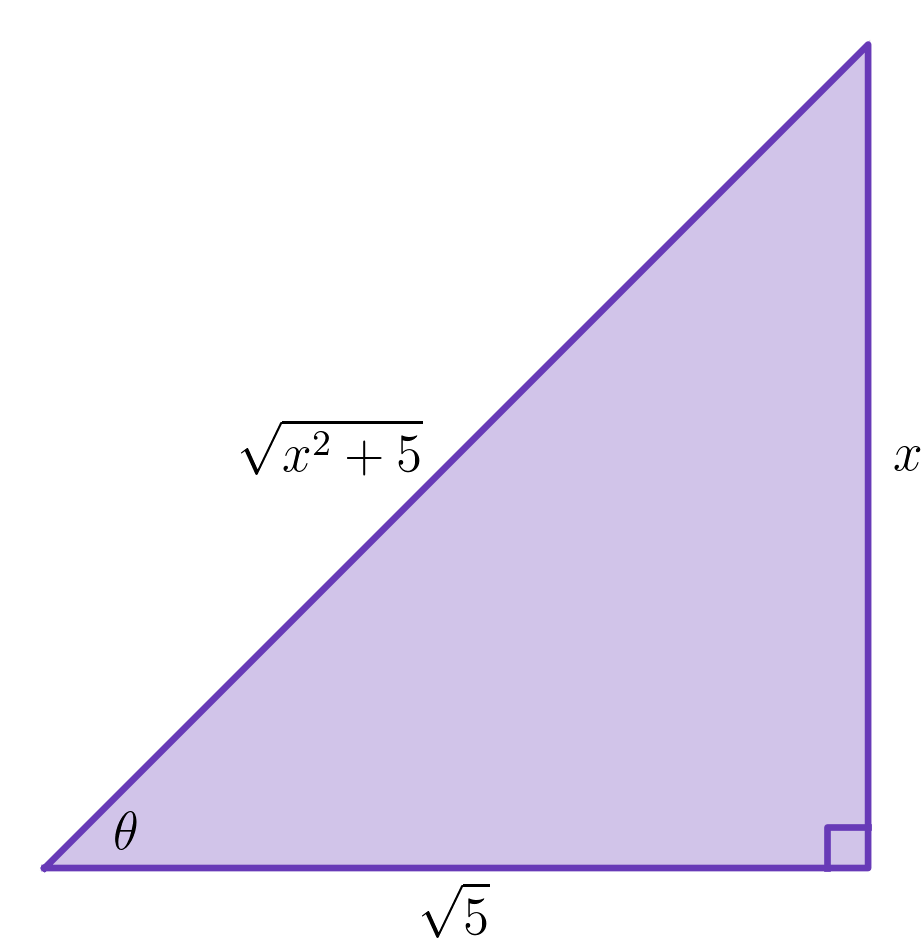
\includegraphics[width=4in]{images/trigsub02.png}
\end{image}
\end{center}
\item Using this reference triangle, we get that
\[ \tan \theta = \frac{x}{\sqrt{5}} \qquad \sec \theta = \answer{ \frac{\sqrt{x^2+5}}{\sqrt{5}}}. \]
Using these formulas, we can write
\[ \ln |\sec \theta + \tan \theta| = \ln \left| \answer{\frac{x}{\sqrt{5}} + \frac{\sqrt{x^2+5}}{\sqrt{5}}} \right| . \]
\item We conclude that
\[ \int \frac{dx}{\sqrt{x^2+5}} = \ln | x + \sqrt{x^2 + 5} | + C. \]
(Note that the factor of $\sqrt{5}$ in the denominator of the logarithm is not necessary when we already have an arbitrary constant $C$ in our answer.)
\end{itemize}
\end{example}

\begin{example}
Compute the indefinite integral
\[ \int \frac{dx}{x^2 \sqrt{x^2 - 3}}. \]
\begin{itemize}
\item The structure of this integrand is adapted to a trigonometric substitution of \wordChoice{\choice[correct]{secant}\choice{sine}\choice[correct]{tangent}} type, so we let $x = \sqrt{3} \answer{\tan \theta}$. This gives $dx = \sqrt{3} \answer{\sec \theta \tan \theta}~d \theta$.
\item We use the identity $\sec^2 \theta = \tan^2 \theta + 1$, the quantity $x^2 - 3$ can be rewritten using our substitution to equal $\answer{3 \tan^2 \theta}$. Therefore
\[ \int \frac{dx}{x^2 \sqrt{x^2 - 3}} = \int \answer{ \frac{\sqrt{3} \sec \theta \tan \theta}{3 \sec^2 \theta \sqrt{3} \tan \theta}} d \theta = \answer{\frac{\sin \theta}{3}} + C.\] 
\item We construct a reference triangle compatible with our substitution. In this case, that means we need a right triangle with an angle $\theta$ which satisfies $x/\sqrt{3} = \sec \theta$:
\begin{center}
\begin{image}
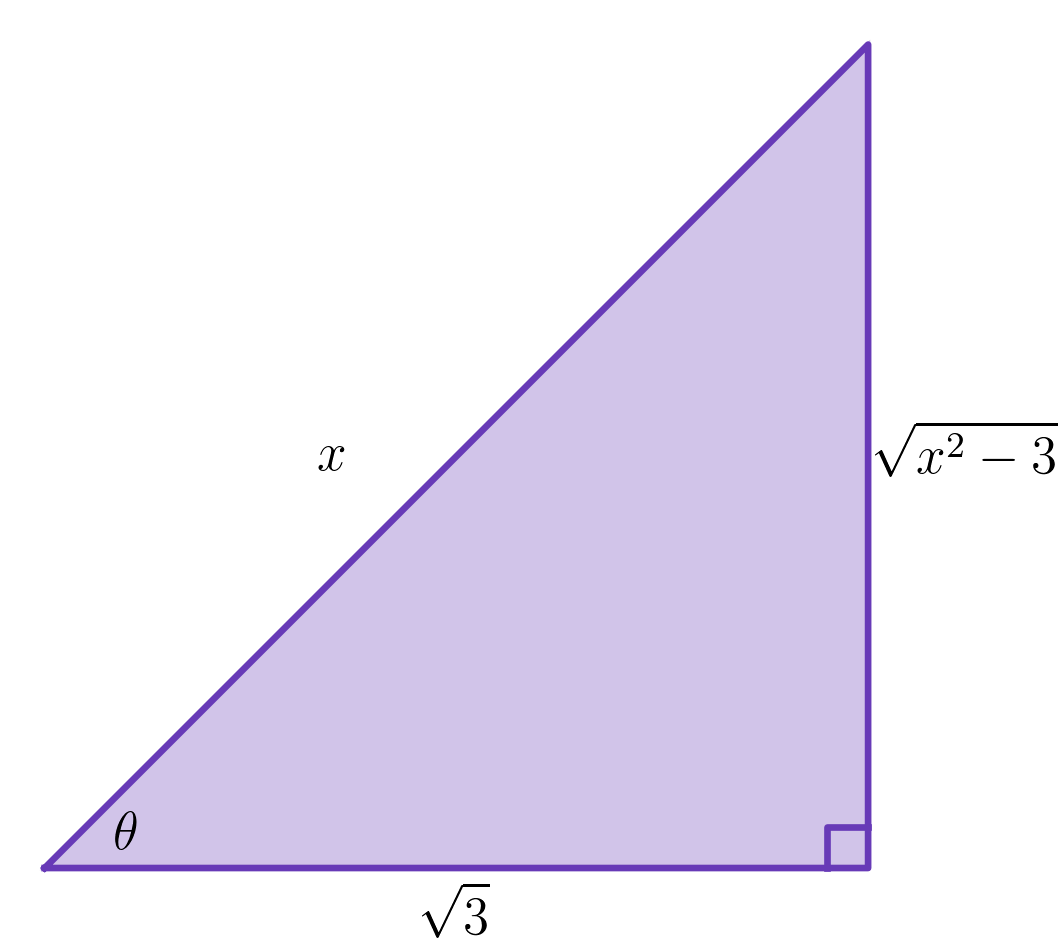
\includegraphics[width=4in]{images/trigsub03.png}
\end{image}
\end{center}
\item Using this reference triangle, we get that
\[ \sin \theta = \answer{\frac{\sqrt{x^2-3}}{x}}.\]
\item We conclude that
\[ \int \frac{dx}{x^2 \sqrt{x^2-3}} = \answer{ \frac{\sqrt{x^2-3}}{3x}} + C. \]
\end{itemize}
\end{example}

\begin{example}
(c.f.~APEX Calculus Example 6.4.1) Compute the indefinite integral
\[ \int \sqrt{9 - x^2} dx. \]
\begin{itemize}
\item The structure of this integrand is adapted to a trigonometric substitution of \wordChoice{\choice{secant}\choice[correct]{sine}\choice{tangent}} type, so we let $x = 3 \answer{\sin \theta}$. This gives $dx = 3 \answer{\cos \theta}~d \theta$.
\item Using the identity $\cos^2 \theta + \sin^2 \theta = 1$, the expression $9 - x^2$ can be rewritten using the formula above as $\answer{(3 \cos \theta)^2}$. Therefore
\[ \int \sqrt{9-x^2} dx = \int \answer{9 (\cos \theta)^2} d \theta. \]
\item We use the power reduction formula $\cos^2 t = (1 + \cos 2t)/2$ and conclude
\[ \int \sqrt{9-x^2} dx = \frac{9}{2} \int \left( 1 + \cos 2 \theta \right) d \theta = \frac{9}{2} \left[ \theta + \frac{1}{2} \sin 2 \theta \right] + C. \]
\item Now we construct a reference triangle which is compatible with the substitution we made. In this case, this means we need a right triangle for which $x/3 = \sin \theta$:
\begin{center}
\begin{image}
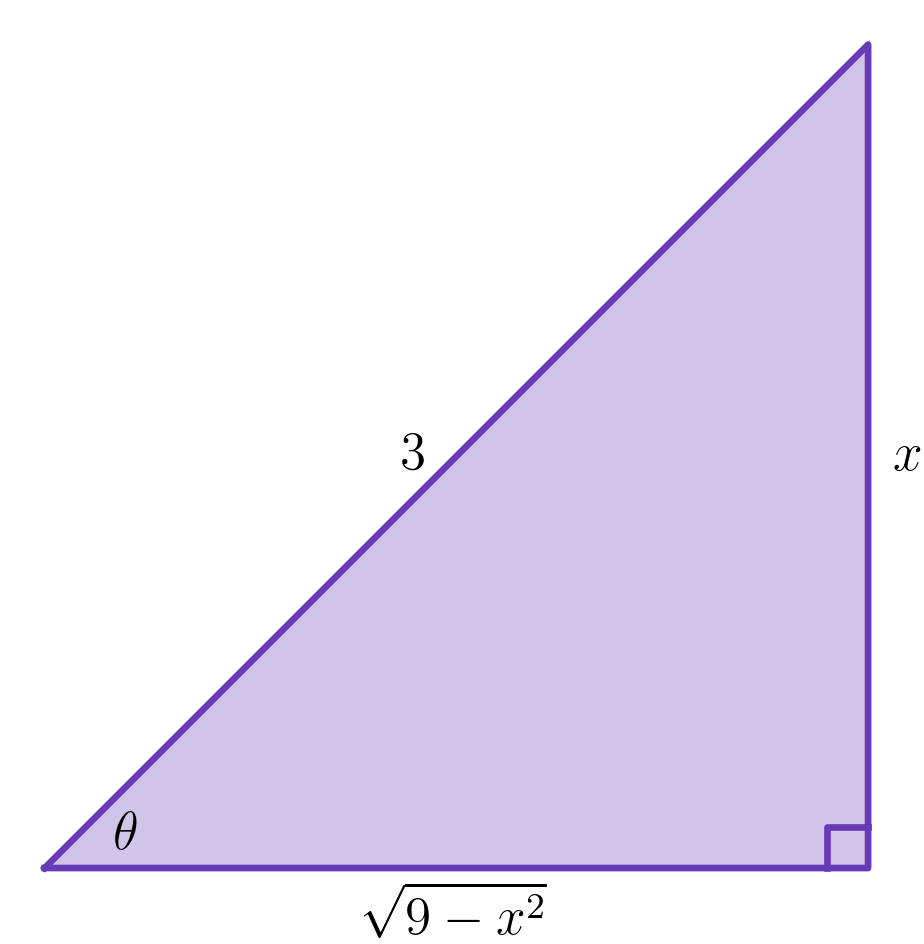
\includegraphics[width=4in]{images/trigsub01.png}
\end{image}
\end{center}
\item Using the reference triangle above, we have the identities
\[ \sin \theta = \frac{x}{3} \qquad \cos \theta = \answer{ \frac{\sqrt{9-x^2}}{3}} \qquad \theta = \arcsin \frac{x}{3}. \]
\item The quantity $\sin 2 \theta$ is difficult to write as a function of $x$ as it stands, so we first use the double-angle formula $\sin 2 \theta = \cos \theta \sin \theta$. We therefore conclude that
\[ \int \sqrt{9-x^2} dx = \answer{ \frac{9}{2} \left( \arcsin \frac{x}{3} + \frac{x \sqrt{9-x^2}}{9} \right)} + C. \]
(Note: Ximera will interpret $\sin^{-1} x$ as $1/(\sin x)$, so write $\arcsin$ when you mean inverse sine.)
\end{itemize}
\end{example}




\end{document}
